% Options for packages loaded elsewhere
\PassOptionsToPackage{unicode}{hyperref}
\PassOptionsToPackage{hyphens}{url}
%
\documentclass[
  man]{apa6}
\usepackage{amsmath,amssymb}
\usepackage{lmodern}
\usepackage{iftex}
\ifPDFTeX
  \usepackage[T1]{fontenc}
  \usepackage[utf8]{inputenc}
  \usepackage{textcomp} % provide euro and other symbols
\else % if luatex or xetex
  \usepackage{unicode-math}
  \defaultfontfeatures{Scale=MatchLowercase}
  \defaultfontfeatures[\rmfamily]{Ligatures=TeX,Scale=1}
\fi
% Use upquote if available, for straight quotes in verbatim environments
\IfFileExists{upquote.sty}{\usepackage{upquote}}{}
\IfFileExists{microtype.sty}{% use microtype if available
  \usepackage[]{microtype}
  \UseMicrotypeSet[protrusion]{basicmath} % disable protrusion for tt fonts
}{}
\makeatletter
\@ifundefined{KOMAClassName}{% if non-KOMA class
  \IfFileExists{parskip.sty}{%
    \usepackage{parskip}
  }{% else
    \setlength{\parindent}{0pt}
    \setlength{\parskip}{6pt plus 2pt minus 1pt}}
}{% if KOMA class
  \KOMAoptions{parskip=half}}
\makeatother
\usepackage{xcolor}
\usepackage{graphicx}
\makeatletter
\def\maxwidth{\ifdim\Gin@nat@width>\linewidth\linewidth\else\Gin@nat@width\fi}
\def\maxheight{\ifdim\Gin@nat@height>\textheight\textheight\else\Gin@nat@height\fi}
\makeatother
% Scale images if necessary, so that they will not overflow the page
% margins by default, and it is still possible to overwrite the defaults
% using explicit options in \includegraphics[width, height, ...]{}
\setkeys{Gin}{width=\maxwidth,height=\maxheight,keepaspectratio}
% Set default figure placement to htbp
\makeatletter
\def\fps@figure{htbp}
\makeatother
\setlength{\emergencystretch}{3em} % prevent overfull lines
\providecommand{\tightlist}{%
  \setlength{\itemsep}{0pt}\setlength{\parskip}{0pt}}
\setcounter{secnumdepth}{-\maxdimen} % remove section numbering
% Make \paragraph and \subparagraph free-standing
\ifx\paragraph\undefined\else
  \let\oldparagraph\paragraph
  \renewcommand{\paragraph}[1]{\oldparagraph{#1}\mbox{}}
\fi
\ifx\subparagraph\undefined\else
  \let\oldsubparagraph\subparagraph
  \renewcommand{\subparagraph}[1]{\oldsubparagraph{#1}\mbox{}}
\fi
\newlength{\cslhangindent}
\setlength{\cslhangindent}{1.5em}
\newlength{\csllabelwidth}
\setlength{\csllabelwidth}{3em}
\newlength{\cslentryspacingunit} % times entry-spacing
\setlength{\cslentryspacingunit}{\parskip}
\newenvironment{CSLReferences}[2] % #1 hanging-ident, #2 entry spacing
 {% don't indent paragraphs
  \setlength{\parindent}{0pt}
  % turn on hanging indent if param 1 is 1
  \ifodd #1
  \let\oldpar\par
  \def\par{\hangindent=\cslhangindent\oldpar}
  \fi
  % set entry spacing
  \setlength{\parskip}{#2\cslentryspacingunit}
 }%
 {}
\usepackage{calc}
\newcommand{\CSLBlock}[1]{#1\hfill\break}
\newcommand{\CSLLeftMargin}[1]{\parbox[t]{\csllabelwidth}{#1}}
\newcommand{\CSLRightInline}[1]{\parbox[t]{\linewidth - \csllabelwidth}{#1}\break}
\newcommand{\CSLIndent}[1]{\hspace{\cslhangindent}#1}
\ifLuaTeX
\usepackage[bidi=basic]{babel}
\else
\usepackage[bidi=default]{babel}
\fi
\babelprovide[main,import]{english}
% get rid of language-specific shorthands (see #6817):
\let\LanguageShortHands\languageshorthands
\def\languageshorthands#1{}
% Manuscript styling
\usepackage{upgreek}
\captionsetup{font=singlespacing,justification=justified}

% Table formatting
\usepackage{longtable}
\usepackage{lscape}
% \usepackage[counterclockwise]{rotating}   % Landscape page setup for large tables
\usepackage{multirow}		% Table styling
\usepackage{tabularx}		% Control Column width
\usepackage[flushleft]{threeparttable}	% Allows for three part tables with a specified notes section
\usepackage{threeparttablex}            % Lets threeparttable work with longtable

% Create new environments so endfloat can handle them
% \newenvironment{ltable}
%   {\begin{landscape}\centering\begin{threeparttable}}
%   {\end{threeparttable}\end{landscape}}
\newenvironment{lltable}{\begin{landscape}\centering\begin{ThreePartTable}}{\end{ThreePartTable}\end{landscape}}

% Enables adjusting longtable caption width to table width
% Solution found at http://golatex.de/longtable-mit-caption-so-breit-wie-die-tabelle-t15767.html
\makeatletter
\newcommand\LastLTentrywidth{1em}
\newlength\longtablewidth
\setlength{\longtablewidth}{1in}
\newcommand{\getlongtablewidth}{\begingroup \ifcsname LT@\roman{LT@tables}\endcsname \global\longtablewidth=0pt \renewcommand{\LT@entry}[2]{\global\advance\longtablewidth by ##2\relax\gdef\LastLTentrywidth{##2}}\@nameuse{LT@\roman{LT@tables}} \fi \endgroup}

% \setlength{\parindent}{0.5in}
% \setlength{\parskip}{0pt plus 0pt minus 0pt}

% Overwrite redefinition of paragraph and subparagraph by the default LaTeX template
% See https://github.com/crsh/papaja/issues/292
\makeatletter
\renewcommand{\paragraph}{\@startsection{paragraph}{4}{\parindent}%
  {0\baselineskip \@plus 0.2ex \@minus 0.2ex}%
  {-1em}%
  {\normalfont\normalsize\bfseries\itshape\typesectitle}}

\renewcommand{\subparagraph}[1]{\@startsection{subparagraph}{5}{1em}%
  {0\baselineskip \@plus 0.2ex \@minus 0.2ex}%
  {-\z@\relax}%
  {\normalfont\normalsize\itshape\hspace{\parindent}{#1}\textit{\addperi}}{\relax}}
\makeatother

\makeatletter
\usepackage{etoolbox}
\patchcmd{\maketitle}
  {\section{\normalfont\normalsize\abstractname}}
  {\section*{\normalfont\normalsize\abstractname}}
  {}{\typeout{Failed to patch abstract.}}
\patchcmd{\maketitle}
  {\section{\protect\normalfont{\@title}}}
  {\section*{\protect\normalfont{\@title}}}
  {}{\typeout{Failed to patch title.}}
\makeatother

\usepackage{xpatch}
\makeatletter
\xapptocmd\appendix
  {\xapptocmd\section
    {\addcontentsline{toc}{section}{\appendixname\ifoneappendix\else~\theappendix\fi\\: #1}}
    {}{\InnerPatchFailed}%
  }
{}{\PatchFailed}
\keywords{prosocial behavior\newline\indent Word count: 97}
\DeclareDelayedFloatFlavor{ThreePartTable}{table}
\DeclareDelayedFloatFlavor{lltable}{table}
\DeclareDelayedFloatFlavor*{longtable}{table}
\makeatletter
\renewcommand{\efloat@iwrite}[1]{\immediate\expandafter\protected@write\csname efloat@post#1\endcsname{}}
\makeatother
\usepackage{lineno}

\linenumbers
\usepackage{csquotes}
\ifLuaTeX
  \usepackage{selnolig}  % disable illegal ligatures
\fi
\IfFileExists{bookmark.sty}{\usepackage{bookmark}}{\usepackage{hyperref}}
\IfFileExists{xurl.sty}{\usepackage{xurl}}{} % add URL line breaks if available
\urlstyle{same} % disable monospaced font for URLs
\hypersetup{
  pdftitle={The Influence of Person-based vs.~Identity-based language on Attitude and Prosocial Behavior},
  pdfauthor={Songyang Zhang1 \& Janet Geipel1,2},
  pdflang={en-EN},
  pdfkeywords={prosocial behavior},
  hidelinks,
  pdfcreator={LaTeX via pandoc}}

\title{The Influence of Person-based vs.~Identity-based language on Attitude and Prosocial Behavior}
\author{Songyang Zhang\textsuperscript{1} \& Janet Geipel\textsuperscript{1,2}}
\date{}


\shorttitle{Influence of Language on Prosocial Behavior}

\authornote{

The authors made the following contributions. Songyang Zhang: Conceptualization, Writing - Original Draft Preparation, Writing - Review \& Editing; Janet Geipel: Writing - Review \& Editing, Supervision.

}

\affiliation{\vspace{0.5cm}\textsuperscript{1} University of Chicago\\\textsuperscript{2} University of Exeter}

\abstract{%
This study examines the influence of language framing on prosocial behavior towards the homeless. It contrasts the effects of identity-based language (``homeless people'', ``unhoused people'') with person-based language (``people who experience homelessness'') on donation intentions and attitudes. Conducted with 32 U.S. English speakers, the experiment employed a between-subjects design, where participants were exposed to varied language framing in a news article context. Measures included hypothetical donation amounts to homelessness support, attitudes towards homeless individuals, and support for relevant government policies. These insights are vital for policymakers and advocates in promoting inclusive discourse and support for marginalized populations.
}



\begin{document}
\maketitle

\hypertarget{introduction}{%
\section{Introduction}\label{introduction}}

Language framing can profoundly influence people's perceptions, attitudes, and behaviors. The concept of framing, as posited by Tversky and Kahneman, illustrates how different presentations of equivalent information can lead to diverse outcomes in decision-making processes (Tversky \& Kahneman, 1981). This principle extends into the realm of prosocial behavior, where language framing of social issues can significantly affect individuals' decisions and willingness to engage in prosocial behavior towards others. Studies in social psychology and behavioral science have consistently demonstrated that shifts in language framing can alter prosocial intentions and actions (Ceylan \& Hayran, 2021) (Granello \& Gibbs, 2016).

In the current study, we focused on the effect of identity-based framing and person-based framing, analyze how such factor influence people's attitude to marginalized group and their prosocial behavior. To be specific, identity-based language focused on one's identity (eg. disabled people, homeless people, etc.), whereas person-based language put the person at the center of language expression (eg. people who experience homelessness, people who have mental illness). By examining the effects of using identity-based language against person-based language, the study seeks to reveal how subtle shifts in language framing can impact empathy, reduce stigma, and influence the willingness to support social causes.

The discourse around identity vs.~person based language framing occurred among various domains, including disability, mental health, and autism, where the preference and criteria for using different language framing are still vastly debated. The American Psychological Association (APA) and other authoritative bodies like the American Medical Association (AMA) and the National Institute of Health (NIH) have traditionally advocated for the use of person-based language to describe individuals with disabilities or conditions, aiming to emphasize the personhood over the their physical and/or mental condition (CDC, 2022), (NIH, 2022), (Dunn \& Andrews, 2015). However, within the disability and autism communities, there's a growing debate between the preference for identity-based language by people within the marginalized community and advocation for person-based language by medical professionals (Buijsman, Begeer, \& Scheeren, 2023), (Taboas, Doepke, \& Zimmerman, 2023).

Despite the ongoing discourse around use of person-based vs.~identity-based language, there has been a gap in empirical research, in which less research has focused on the effect of language on people's perception and prosocial behavior outcomes. Furthermore, much of the existing literature has focused on specific areas like disability or mental health, without exploring the broader implications of these findings for other social issues, including homelessness. Thus, the current research focused specifically within the context of homelessness, analyzing the effect of identity-based and person-based language on people's general attitude and prosocial donation behavior.

The current research offers a more comprehensive understanding in language-framing and prosocial behavior within the context of homelessness. Through the experimental manipulation of language framing, we are able to gain insight to the causal consequence of language framing and subsequently measuring its impact on participants' donation intentions. This research also provides a more integrated theoretical framework for understanding the role of language in social issues. It can provide practical guidance for policymakers in crafting more effective information to gain support for marginalized populations, thereby supporting more inclusive public discourse.

\hypertarget{methods}{%
\section{Methods}\label{methods}}

\hypertarget{study-design}{%
\subsection{Study Design}\label{study-design}}

The current study used between-subjects design, where participants were randomly assigned to one of three language framing conditions: identity-based language (``homeless people''), identity-based language (``unhoused people''), and person-based language (``people who experience homelessness''). The primary dependent variable was the participants' willingness to engage in prosocial behavior (how much are they likely to donate their money out of 100 dollars to support the targeted population if they win lottery)

\hypertarget{participants}{%
\subsection{Participants}\label{participants}}

We recruited 33 native English speakers from the U.S. on Prolific (age range: 18 to 67, Mage = 42.97 years, \emph{SD} = 13; 52\% male, 48\% female). Participants received 9 pounds/hour. On average they needed 7 minutes to complete the study. Participants were randomly assigned to one of three labelling groups: unhoused people (\emph{n} = 10), homeless people (\emph{n} = 12), people who experience homelessness (\emph{n} = 11). We excluded one participant as they had a duplicated IP address and Prolific ID. The final sample consists of 32 participants.

\hypertarget{procedure}{%
\subsection{Procedure}\label{procedure}}

After providing informed consent, participants read a news article about an organization aiming to find affordable housing for people who experience homelessness. Within the news article, we varied the language-framing that is referring to people who experience homelessness/unhoused people/homeless people. Participants were informed that the study aims to understand how informative online news articles are.

\hypertarget{measures}{%
\subsection{Measures}\label{measures}}

\hypertarget{recognition-measure}{%
\subsubsection{Recognition Measure}\label{recognition-measure}}

The participants were first asked to answer three recognition check for the online news article. The three multiple choice question asked: ``who is Dan Valdez?'', ``what is the main goal of Brilliant Corners'', and ``what is a major issue in Los Angeles mentioned in the article?''. The recognition measure were developed based on the content of the news article, and the answers were obvious if the participants carefully read the article.

\hypertarget{article-perception-measure}{%
\subsubsection{Article Perception Measure}\label{article-perception-measure}}

The participants were asked to report their perception of the online news article in five dimensions (informative, understandable, interesting, read in detail, concentration), in which the five item survey was measured through 7-point Likert scale (0 = \emph{Not at all}, 6 = \emph{Very}).

\hypertarget{donation-intention}{%
\subsubsection{Donation Intention}\label{donation-intention}}

Participants were presented with a hypothetical scenario where they could win 100 dollar in a study lottery and were asked how much they would like to donate to support the homeless population, with options ranging from 0 dollar to 100 dollars.

\hypertarget{attitude-measure}{%
\subsubsection{Attitude Measure}\label{attitude-measure}}

Participants reported their thoughts and feelings about the homeless population through several statements related to mental and material resources, dishonesty, and other dimensions. Responses were captured on a 7-point Likert scale from 1 (\emph{strongly disagree}) to 7 (\emph{strongly agree}). The attitude measure is adapted from measures of stigmatization scale (Newman, Tang, \& Bakina, 2022).

\hypertarget{tax-support-for-housing-program}{%
\subsubsection{Tax Support for Housing Program}\label{tax-support-for-housing-program}}

Participants were asked about their willingness to pay extra taxes for a ``Housing-for-all'' program from 0 (\emph{Very unlikely}) to 6 (\emph{Very likely}) and their general support for such a program, indicated by binary measure of yes or no.

\hypertarget{government-support-and-policy-measures}{%
\subsubsection{Government Support and Policy Measures}\label{government-support-and-policy-measures}}

Questions in this section explored the perceived priority of government support for homeless individuals and willingness to sign a petition for initiatives to help the homeless population. Responses varied from 0 (\emph{very low priority}) to 6 (\emph{very high priority}) for budget priorities and 0 to 100 for petition signing willingness.

\hypertarget{demographics}{%
\subsubsection{Demographics}\label{demographics}}

Participants provided information on age, ethnicity, education level, employment status, and annual household income.

\hypertarget{data-analysis}{%
\subsection{Data analysis}\label{data-analysis}}

We used R (Version 4.2.3; R Core Team, 2023) and the R-packages \emph{dplyr} (Version 1.1.0; Wickham, François, Henry, Müller, \& Vaughan, 2023), \emph{forcats} (Version 1.0.0; Wickham, 2023), \emph{ggplot2} (Version 3.4.2; Wickham, 2016), \emph{ggsci} (Version 3.0.0; Xiao, 2023), \emph{lubridate} (Version 1.9.2; Grolemund \& Wickham, 2011), \emph{papaja} (Version 0.1.2; Aust \& Barth, 2023), \emph{purrr} (Version 1.0.1; Wickham \& Henry, 2023), \emph{readr} (Version 2.1.4; Wickham, Hester, \& Bryan, 2023), \emph{stringr} (Version 1.5.0; Wickham, 2022), \emph{tibble} (Version 3.2.1; Müller \& Wickham, 2023), \emph{tidyr} (Version 1.3.0; Wickham, Vaughan, \& Girlich, 2023), \emph{tidyverse} (Version 2.0.0; Wickham et al., 2019), and \emph{tinylabels} (Version 0.2.4; Barth, 2023) for all our analyses.

\hypertarget{results}{%
\section{Results}\label{results}}

\hypertarget{participants-demographics}{%
\subsection{Participants Demographics}\label{participants-demographics}}

We recruited 33 native English speakers from the U.S. on Prolific (age range: 18 to
67, Mage = 44 years, SD = 13; 52\% male, 48\% female). Participants received 9
pounds/hour. On average they needed 7 minutes to complete the study. Participants
were randomly assigned to one of three labelling groups: unhoused people (n = 10),
homeless people (n = 12), people who experience homelessness (n = 11). We
excluded one participant as they had a duplicated IP address and Prolific ID. The final
sample consists of 32 participants. In terms of education, 28.1\% of participants
indicated to have a high school degree, 28.1\% associate's degree, 31.3\% a bachelor's
degree, and 12.5\% a master's degree. In terms of employment status, 56.3\% of
participants indicated to have a full-time employment status, 18.8\% a part-time, 15.6\%
unemployed, 9.4\% not employed. In terms of ethnicity, 72\% of participants indicated
to be white, 22\% to be black or African American, and 6\% Hispanic.

For a detailed account for the demographics of participants by each condition, see table included in the supplementary material.

\begin{table}
\centering
\caption{\label{tab:my-table}Summary of Demographic Variables by Condition}
\centering
\resizebox{\ifdim\width>\linewidth\linewidth\else\width\fi}{!}{
\begin{tabular}[t]{l|r|r|r|r|r}
\hline
Condition & Avg\_Age & Avg\_Political\_Economy\_Issue & Avg\_Political\_Social\_Issue & Avg\_Education\_Level & Avg\_Employment\_Status\\
\hline
homeless people & 37.16667 & 3.583333 & 3.583333 & 2.833333 & 2.083333\\
\hline
people who experience homelessness & 47.72727 & 3.454546 & 3.363636 & 3.181818 & 1.818182\\
\hline
unhoused people & 44.88889 & 3.777778 & 3.333333 & 4.000000 & 2.222222\\
\hline
\end{tabular}}
\end{table}

\hypertarget{recognition-measure-1}{%
\subsection{Recognition Measure}\label{recognition-measure-1}}

30 out of 32 participants (93.8\%) passed the first recognition test (``Who is Dan Valdez?'' {[}a{]} A landlord in Los Angeles, {[}b{]} An advocate for luxury housing, {[}c{]} A team member at Brilliant Corners, {[}d{]} The mayor of Los Angeles.). All 32 participants (100\%) passed the second (``What is the main goal of Brilliant Corners?'' {[}a{]} Building new apartments, {[}b{]} Finding homes for unhoused people {[}people who are homeless, homeless people{]}, {[}c{]} Providing job training, {[}d{]} Offering medical assistance) and all participants (100\%) passed the third recognition test (``What is a major issue in Los Angeles mentioned in the article?'' {[}a{]} Lack of public transportation, {[}b{]} Shortage of affordable housing, {[}c{]} High crime rates, {[}d{]} Pollution).

\hypertarget{article-perception-measure-1}{%
\subsection{Article Perception Measure}\label{article-perception-measure-1}}

On average, participants perceived the article as informative (\(M\) = 4.84, \(SD\) = 1.27, scale: 1 = \emph{not at all informative} to 6 = \emph{very informative}), understandable (\(M\) = 5.47, \(SD\) = 0.67, scale: 1 = \emph{not at all understandable} to 6 = \emph{very understandable}), and as interesting (\(M\) = 4.25, \(SD\) = 1.52, scale: 1 = \emph{not at all interesting} to 6 = \emph{very interesting}). On average, participants indicated that they read the article well and in detail (\(M\) = 5.44, \(SD\) = 0.98, scale: 1 = \emph{not at all well} to 6 = \emph{very well and in detail}) and that it was not difficult to read the news article (\(M\) = 1.75, \(SD\) = 1.97, scale: 0 = \emph{not at all difficult} to 6 = \emph{very difficult}).

\hypertarget{donation-intention-1}{%
\subsection{Donation Intention}\label{donation-intention-1}}

The main dependent variable that we are interested in here is the donation intention, in which we asked the participants to report their intention to donate to support homeless people, unhoused people, or people who experience homeless, out of 100 dollar. A one-way ANOVA was conducted to examine the impact of language framing on participants' intention to donate intention. The analysis revealed that language framing did not significantly affect donation intentions, \(F\)(2, 29) = 0.61, \(p\) = 0.55, with a mean square between groups (Condition) of 463.32 and a mean square within groups (error) of 753.64.

The graph below shows the donation intention by condition.
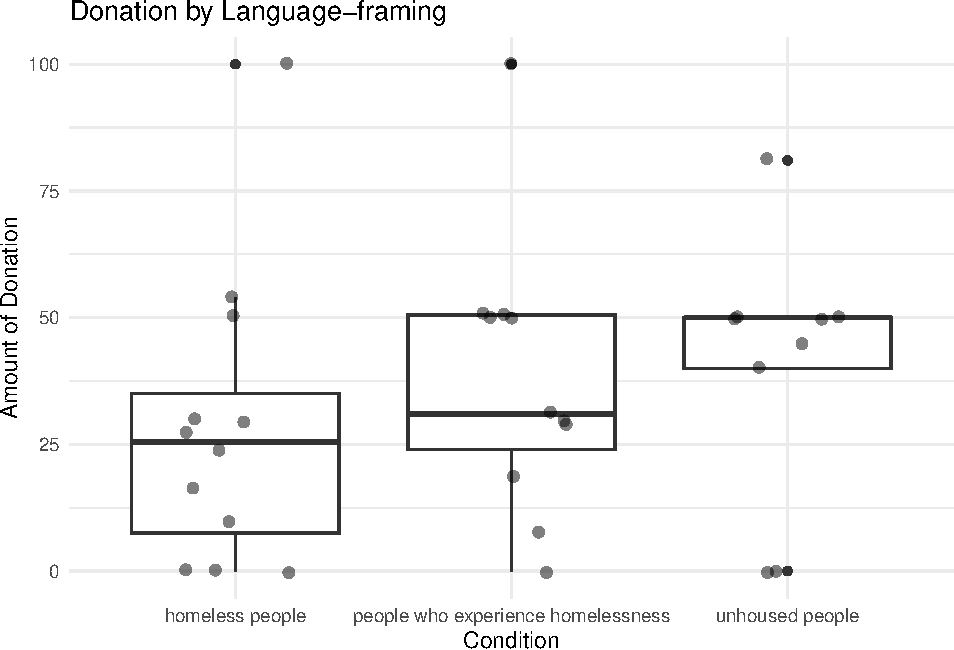
\includegraphics{d2m_final-project_files/figure-latex/unnamed-chunk-3-1.pdf}

\hypertarget{support-for-housing-for-all-program}{%
\subsection{Support for Housing for All Program}\label{support-for-housing-for-all-program}}

Then, we are interested in the whether the secondary outcome measure, support for housing for all program (scale: 0 = \emph{Not at all}, 6 = \emph{Very much}), differ across different language framing conditions. A one-way anova was conducted, revealing that the effect of language framing on support for housing-for-all program is no statistically significant (\(F\)(2, 29) = 0.941, \(p\) = .402). The bar graph below shows the mean of support for housing-for-all program across conditions.

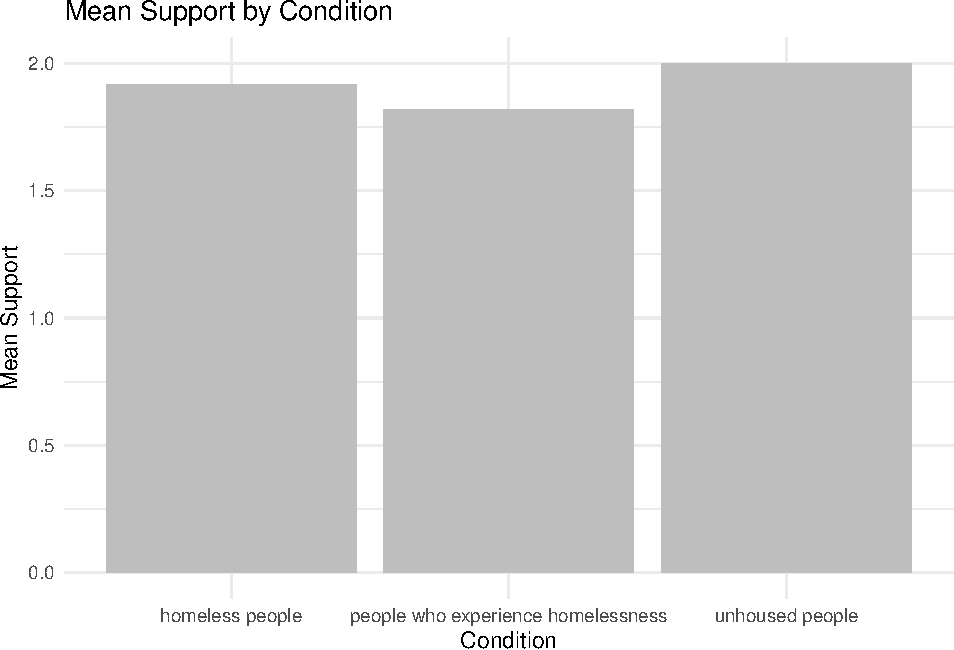
\includegraphics{d2m_final-project_files/figure-latex/unnamed-chunk-5-1.pdf}

\hypertarget{discussion}{%
\section{Discussion}\label{discussion}}

The current study examine the influence of language framing on prosocial behaviors, specifically donation intentions, and support for housing initiatives. The findings from the one-way ANOVA analyses suggest language framing does not significantly impact donation intentions or support for a ``housing for all'' program.

One possible explanation for the non-significant result is the small sample size. In the current pilot study, there are only 32 participants, meaning approximately 10 participants within each condition. As a result, with the small sample size in the study, we might not detect any significant differences in donation amount. For future study, we will include more participants to see if there is a significant differences among language-framing conditions.

The current study design contributes to the ongoing discourse on the influence of language-framing on prosocial intention and behavior. Future studies could explore more diverse language frames with larger sample size to have enough effect size to detect significance result. The person-based and identity-based framing is also being used in different context beyond homelessness. Possible future research can analyze the influence of language-framing to different marginalized group.

\newpage

\hypertarget{references}{%
\section{References}\label{references}}

\hypertarget{refs}{}
\begin{CSLReferences}{1}{0}
\leavevmode\vadjust pre{\hypertarget{ref-R-papaja}{}}%
Aust, F., \& Barth, M. (2023). \emph{{papaja}: {Prepare} reproducible {APA} journal articles with {R Markdown}}. Retrieved from \url{https://github.com/crsh/papaja}

\leavevmode\vadjust pre{\hypertarget{ref-R-tinylabels}{}}%
Barth, M. (2023). \emph{{tinylabels}: Lightweight variable labels}. Retrieved from \url{https://cran.r-project.org/package=tinylabels}

\leavevmode\vadjust pre{\hypertarget{ref-buijsman_autistic_2023}{}}%
Buijsman, R., Begeer, S., \& Scheeren, A. M. (2023). '{Autistic} person' or 'person with autism'? {Person}-first language preference in {Dutch} adults with autism and parents. \emph{Autism: The International Journal of Research and Practice}, \emph{27}(3), 788--795. \url{https://doi.org/10.1177/13623613221117914}

\leavevmode\vadjust pre{\hypertarget{ref-cdc_cdcs_2022}{}}%
CDC. (2022). {CDC}'s {Key} {Principles} for {Inclusive} {Communication}. Retrieved from \url{https://www.cdc.gov/healthcommunication/Key_Principles.html}

\leavevmode\vadjust pre{\hypertarget{ref-ceylan_message_2021}{}}%
Ceylan, M., \& Hayran, C. (2021). Message {Framing} {Effects} on {Individuals}' {Social} {Distancing} and {Helping} {Behavior} {During} the {COVID}-19 {Pandemic}. \emph{Frontiers in Psychology}, \emph{12}. Retrieved from \url{https://www.frontiersin.org/journals/psychology/articles/10.3389/fpsyg.2021.579164}

\leavevmode\vadjust pre{\hypertarget{ref-dunn_person-first_2015}{}}%
Dunn, D. S., \& Andrews, E. E. (2015). Person-first and identity-first language: {Developing} psychologists' cultural competence using disability language. \emph{American Psychologist}, \emph{70}(3), 255--264. \url{https://doi.org/10.1037/a0038636}

\leavevmode\vadjust pre{\hypertarget{ref-granello_power_2016}{}}%
Granello, D. H., \& Gibbs, T. A. (2016). The {Power} of {Language} and {Labels}: {``{The} {Mentally} {Ill}''} {Versus} {``{People} {With} {Mental} {Illnesses}.''} \emph{Journal of Counseling \& Development}, \emph{94}(1), 31--40. \url{https://doi.org/10.1002/jcad.12059}

\leavevmode\vadjust pre{\hypertarget{ref-R-lubridate}{}}%
Grolemund, G., \& Wickham, H. (2011). Dates and times made easy with {lubridate}. \emph{Journal of Statistical Software}, \emph{40}(3), 1--25. Retrieved from \url{https://www.jstatsoft.org/v40/i03/}

\leavevmode\vadjust pre{\hypertarget{ref-R-tibble}{}}%
Müller, K., \& Wickham, H. (2023). \emph{Tibble: Simple data frames}. Retrieved from \url{https://CRAN.R-project.org/package=tibble}

\leavevmode\vadjust pre{\hypertarget{ref-newman_general_2022}{}}%
Newman, L., Tang, Y., \& Bakina, D. A. (2022). A general, theory-based measure of stigmatization (the {GEMS}): {Development} and an application. \emph{Evolutionary Psychological Science}, \emph{8}(1), 30--45. \url{https://doi.org/10.1007/s40806-021-00309-6}

\leavevmode\vadjust pre{\hypertarget{ref-nih_person-first_2022}{}}%
NIH. (2022). Person-first and {Destigmatizing} {Language}. Retrieved from \url{https://www.nih.gov/nih-style-guide/person-first-destigmatizing-language}

\leavevmode\vadjust pre{\hypertarget{ref-R-base}{}}%
R Core Team. (2023). \emph{R: A language and environment for statistical computing}. Vienna, Austria: R Foundation for Statistical Computing. Retrieved from \url{https://www.R-project.org/}

\leavevmode\vadjust pre{\hypertarget{ref-taboas_preferences_2023}{}}%
Taboas, A., Doepke, K., \& Zimmerman, C. (2023). Preferences for identity-first versus person-first language in a {US} sample of autism stakeholders. \emph{Autism: The International Journal of Research and Practice}, \emph{27}(2), 565--570. \url{https://doi.org/10.1177/13623613221130845}

\leavevmode\vadjust pre{\hypertarget{ref-tversky_framing_1981}{}}%
Tversky, A., \& Kahneman, D. (1981). The framing of decisions and the psychology of choice. \emph{Science}, \emph{211}(4481), 453--458. \url{https://doi.org/10.1126/science.7455683}

\leavevmode\vadjust pre{\hypertarget{ref-R-ggplot2}{}}%
Wickham, H. (2016). \emph{ggplot2: Elegant graphics for data analysis}. Springer-Verlag New York. Retrieved from \url{https://ggplot2.tidyverse.org}

\leavevmode\vadjust pre{\hypertarget{ref-R-stringr}{}}%
Wickham, H. (2022). \emph{Stringr: Simple, consistent wrappers for common string operations}. Retrieved from \url{https://CRAN.R-project.org/package=stringr}

\leavevmode\vadjust pre{\hypertarget{ref-R-forcats}{}}%
Wickham, H. (2023). \emph{Forcats: Tools for working with categorical variables (factors)}. Retrieved from \url{https://CRAN.R-project.org/package=forcats}

\leavevmode\vadjust pre{\hypertarget{ref-R-tidyverse}{}}%
Wickham, H., Averick, M., Bryan, J., Chang, W., McGowan, L. D., François, R., \ldots{} Yutani, H. (2019). Welcome to the {tidyverse}. \emph{Journal of Open Source Software}, \emph{4}(43), 1686. \url{https://doi.org/10.21105/joss.01686}

\leavevmode\vadjust pre{\hypertarget{ref-R-dplyr}{}}%
Wickham, H., François, R., Henry, L., Müller, K., \& Vaughan, D. (2023). \emph{Dplyr: A grammar of data manipulation}. Retrieved from \url{https://CRAN.R-project.org/package=dplyr}

\leavevmode\vadjust pre{\hypertarget{ref-R-purrr}{}}%
Wickham, H., \& Henry, L. (2023). \emph{Purrr: Functional programming tools}. Retrieved from \url{https://CRAN.R-project.org/package=purrr}

\leavevmode\vadjust pre{\hypertarget{ref-R-readr}{}}%
Wickham, H., Hester, J., \& Bryan, J. (2023). \emph{Readr: Read rectangular text data}. Retrieved from \url{https://CRAN.R-project.org/package=readr}

\leavevmode\vadjust pre{\hypertarget{ref-R-tidyr}{}}%
Wickham, H., Vaughan, D., \& Girlich, M. (2023). \emph{Tidyr: Tidy messy data}. Retrieved from \url{https://CRAN.R-project.org/package=tidyr}

\leavevmode\vadjust pre{\hypertarget{ref-R-ggsci}{}}%
Xiao, N. (2023). \emph{Ggsci: Scientific journal and sci-fi themed color palettes for 'ggplot2'}. Retrieved from \url{https://CRAN.R-project.org/package=ggsci}

\end{CSLReferences}


\end{document}
